
%%% Local Variables:
%%% mode: latex
%%% TeX-master: t
%%% End:

\chapter{硬件资源共享管理方法}
\label{chap:hwresman}

由于缺少有效的硬件资源共享管理机制,现有服务器体系结构不能很好的在共享场景中工作:
不同应用无管理的访问共享硬件资源,产生资源竞争并造成严重的性能干扰,进而影响应用性能。
大量研究尝试解决不同硬件层次上干扰所带来的性能问题,
如Cache容量划分\cite{kasture_ubik:_2014, sanchez_vantage:_2011, sanchez_zcache:_2010, qureshi_utility-based_2006}
或访存调度\cite{muralidhara_reducing_2011}等。
但受到数据中心海量应用\cite{Reiss_googletrace_2012}且用组合不断变化的特征影响,
这些方法在数据中心内并没有发挥应有的作用,主要有3个方面的原因。
首先,这此方法通常只针对单一硬件资源的竞争,而数据中心应用会在不同的硬件层次上产生竞争;
第二,由于没有统一的框架与接口,无法通过多种方法组合的方式解决不同硬件层次上的竞争;
最后,为每一种可能的硬件资源竞争场景都单独设计一种资源管理方法,
在数据中心这种海量应用的通用场景下是不切实际的。

基于以上3个问题,本章提出一种通用硬件资源管理方法与架构,
通过统一的接口将不同的硬件上不同的机制、策略结合,
使用软件可编程的方式对硬件资源管理方法进行调整,
包括基于``控制平面''的策略可编程和``数据平面''的机制可编程,
以支持数据中心复杂多变的应用场景。
具体内容安排如下:
首先分析通用硬件资源管理的动机,然后针对2类主要硬件资源Cache和内存控制器分析其资源抽象,
提出基于``控制平面''与``数据平面''抽象的资源抽象方法,
具体设计控制平面与数据平面,并使用模拟器对控制平面的效果进行评估,
数据平面由于性能问题无法使用模拟器进行评估,将在第7章中使用FPGA 原型对其进行评估。


\section{问题分析}

\begin{figure}[tb]
  \centering
  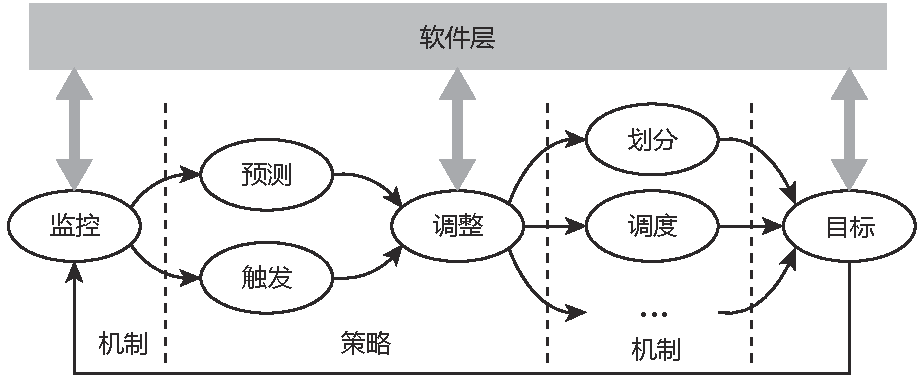
\includegraphics[width=0.8\textwidth]{hwres/resource-manage-flow}
  \caption{资源管理流程模型}
  \label{fig:resource-manage-flow}
\end{figure}

在计算机系统中,通常使用反馈调节的方式实现应用服务质量保障。
根据应用的服务质量需求制定调节目标,可能是单目标或复合的多目标;
采集系统中与目标相关的状态信息,通过预测或条件触发的方式对可能发生的违例进行监控;
当违例发生时,或预测到即将发生违例时,通过调节机制对资源进行重新分配,使系统满足目标。
该过程如图\ref{fig:resource-manage-flow}所示,
除以上所述流程外,通常应用层还会提供目标、监控与调整的接口,用于对整个流程进行控制。

%基于该模型,现有部分软件层次的工作\cite{controlwave2002, Hoffmann:2015, Hoffmann:2014}
%设计了不同的反馈调节机制,实现以QoS或能耗为目标的资源管理,
%本节主要关注如何在硬件体系结构层次利用该模型实现QoS保障的资源管理。

现有服务质量保障工作都是以该模型为基础进行设计。
以Intel RDT技术(参见第\ref{chap:labeladdrspace:intel-rdt}节)为例,
它通过CMT与MBM技术提供处理器末级缓存容量、访存带宽的监控,
在软件层次根据监控结果对资源分配进行调度,
最后通过资源调整接口实现资源重新分配,
目前RDT只提供了CAT技术实现处理器末级缓存容量的划分。
考查其他软硬件服务质量保障技术\cite{tang_reqos:_2013,yang_bubble-flux:_2013,Zhang:2009,herdrich_rate-based_2009,Jigsaw:2013,kasture_ubik:_2014,Nesbit:2006,mutlu_stall-time_2007},
它们虽然针对不同的硬件资源、提供不同机制或策略,
但它们都符合图\ref{fig:resource-manage-flow}所示的资源管理流程模型,
表\ref{tab:resman-compare}列举了这些工作与模型的映射关系。

\begin{table}[htb]
  \centering
  \begin{minipage}[t]{\linewidth}
  \caption{资源管理相关工作}
  \label{tab:resman-compare}
    \begin{tabular*}{\linewidth}{ccp{2cm}p{6cm}}
      \toprule[1.5pt]
      \textbf{相关工作}                        & \textbf{QoS指标} & \textbf{监控机制}   & \textbf{QoS保障策略}     \\
      \midrule[1pt]
      ReQoS\cite{tang_reqos:_2013}             & IPC              & 性能计数器 & 基于编译和运行时的应用执行管控(throttling)     \\
      Bubble Flux\cite{yang_bubble-flux:_2013} & IPC              & 性能计数器 & 基于Linux信号(SIGSTOP \& SIGCONT)的执行管控    \\
      \hline
      Zhang \emph{et.al.}\cite{Zhang:2009}     & 执行时间         & \emph{N/A} & 硬件执行管控,\emph{e.g.} duty-cycle modulation  \\
      Rate-Based QoS\cite{herdrich_rate-based_2009} & IPC、执行时间    & 性能计数器 & 硬件执行管控,\emph{e.g.} clock modulation, DVFS \\
      Intel RDT\cite{intel-rdt}                & 缺失率、带宽     & CMT、MBM                               & Cache容量划分,CAT                                 \\
      Jigsaw\cite{Jigsaw:2013}, Ubik\cite{kasture_ubik:_2014} & 缺失率、长尾延迟 & UMON\cite{qureshi_utility-based_2006}  & Cache容量划分,Vantage\cite{sanchez_vantage:_2011} \\
      FQ-VT\cite{Nesbit:2006}                  & IPC、访存延迟        & \emph{N/A}  & Fair-Queuing访存调度    \\
      STFM\cite{mutlu_stall-time_2007}         & 访存带宽、延迟       & \emph{N/A}  & Stall-Time Fair访存调度 \\
      \bottomrule[1.5pt]
    \end{tabular*}\\[2pt]
  \end{minipage}
\end{table}

虽然以上这些方法具有相同的资源管理模型,在监控与调整方面有通用的地方,
但由于接口问题无法共存。
同时这些方法都只能用于某些特定的场景,
在数据中心这种应用众多且需求各异的通用场景下,任何单一的方法都无法适用。
在这种情况下,为服务器提供多种机制和策略,对它们进行统一的管理,
根据应用负载的不同,选择适当的机制或策略的组合是更为合适的方案。
但由于缺少统一的接口现有方案无法进行统一管理,更不能实现协同工作。

该问题与网络领域中网络设备管理存在相似性。
例如交换机、路由器等网络设备,虽然其具有相同的``存储$\rightarrow$转发''功能模型,
但不同厂商生产的网络设备相互之间并不兼容,由于接口、协议等问题不能协同工作。
而SDN/OpenFlow的出现,为这些网络设备提供了统一的管理协议(OpenFlow),
不同的网络设备可以协同工作,并通过SDN在统一的控制平面对整个网络进行管理;
同时利用SDN可编程特性,可以灵活部署新的策略,并根据应用变化调整网络。
使得网络资源的管理更为灵活。

在体系结构内,不同的硬件部件相当于不同网络设备,需要一个统一架构实现资源管理,
该架构需要具有以下特性:

\begin{enumerate}[leftmargin=2\parindent, nolistsep, label=\arabic*)]
  \item 能够适应不同类型的硬件资源
  \item 能够很容易的集成现有资源管理机制与策略
  \item 灵活的可编程策略实现
  \item 灵活的可编程机制实现
\end{enumerate}

本章所提出的通用硬件资源管理方法使用``控制平面''和``数据平面''抽象描述所有硬件资源(特性1,第\ref{chap:hwresman:res}节),
通过基于控制表的可编程控制平面实现策略可编程(特性3,第\ref{chap:hwresman:cp}节),
通过基于处理器的可编程数据平面实现机制可编程(特性4,第\ref{chap:hwresman:dp}节),
现有的资源管理机制可通过数据平面集成到系统中,而资源管理策略可通过控制平面实现集成(特性2)。



\section{硬件资源抽象}
\label{chap:hwresman:res}

% 硬件资源的``控制平面''与``数据平面''抽象
计算机内的硬件资源主要可以分为两类,一类是基于容量的资源,一类是基于流量的资源。
例如,共享缓存、处理器核、以及硬盘空间是基于容量的资源,
总线带宽、访存带宽、或网络带宽是基于流量的资源。
为了实现对这些硬件资源的管理,PARD将计算机内这些硬件资源抽象为数据平面与控制平面两部分。
其中数据平面用于执行请求操作,如处理器末级缓存对DataArray/TagArray的管理、替换策略实现等;
对于内存控制器,其数据平面负责接收上层访存请求、将物理地址转换为DRAM地址以及访存请求调度等。
而控制平面用于对数据平面的策略进行管理,例如对处理器末级缓存数据平面中替换策略的管理、命中信息统计;
内存控制器数据平面的地址映射与调度策略则是由控制平面进行管理。

% 控制平面与数据平面分离:控制平面是策略接口的抽象,数据平面的机制的实现
数据平面基于硬件原有功能实现,并在此基础上提供机制的可配置功能,
将更多的硬件细节通过控制平面暴露给软件进行管理;
控制平面对数据平面所提供的机制进行管理,如提供监控信息的访问、资源调整的接口,
同时为上层提供策略编程接口,如资源访问冲突发现与预测功能。
通过这种抽象方法,将硬件的资源管理机制与具体的策略分离,
针对数据中心应用数量众多且组合多变的需求,可以在硬件上实现多种资源管理机制(如监控、
划分、调度等),并通过软件可编程的方式实现不同的策略以应对不同的应用需求。

% 静态数据平面设计不能很好的适应数据中心多变的场景
以上方案中,控制平面的可编程主要体现在其对数据平面所提供功能的控制,
而数据平面所提供的功能在其设计完成后即已确定,如果需要增加额外的功能,
则需要对数据平面进行重新的设计,并对控制平面暴露相应的接口。
因此,控制平面的可编程能力受到数据平面所能提供功能的限制。
然而在实际数据中心场景中,应用会对底层的硬件不断提出不同的需求,
如更换处理器末级缓存替换策略、更改内存控制器的地址映射方式与调度策略、
为I/O控制器增加数据加密或压缩的功能等。
静态的数据平面设计不能很好的满足这类需求,需要修改其硬件逻辑才能实现,
而这需要很长的周期,无法适应数据中心这种需要不断变化的场景。

% 通过在数据平面也增加可编程机制,更灵活的资源管理
在学术界中,已有一些研究通过在硬件上增加可编程机制,
实现根据应用需求对硬件策略进行调整的功能。
如体系结构领域已经提出在内存控制器\cite{bojnordi_pardis:_2012, martin2009, kornaros2003}、
Cache与一致性协议\cite{kuskin1994, reinhardt1994, impulse1999, pong1998}
上使用可编程逻辑来提供更灵活的功能,
但这些只考虑了如何为单一应用提供更多的可编程支持,
不能很好的在数据中心这种多应用场景下使用。
在网络领域中也有工作提出在SDN数据平面上增加可编程逻辑的方案,
以提高SDN数据平面的可编程性\cite{p4_2014, song2013, jeyakumar2013, sivaraman2013},
通过数据平面的重编程,达到对更多数据包的检测与处理的目的。
考查现有硬件部件的实现,它们通常使用多阶段流水的方式对输入请求进行处理,
可以借鉴现有这些研究的方法,使用可编程机制替代硬件资源中部分流水级,
使用执行固件代码的方式对硬件部件的请求进行处理,
并通过更新数据平面处理器固件的方式实现数据平面功能的扩展,
以增强计算机体系结构的可编程灵活度,
使其能够适应更加复杂多变的数据中心应用场景。

\begin{figure}[tb]
  \centering
  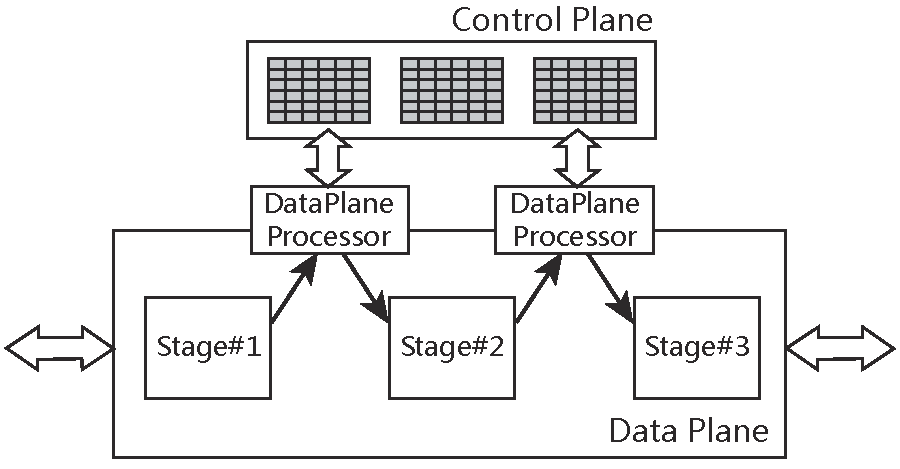
\includegraphics[width=0.6\textwidth]{hwres/pard-res-abstract}
  \caption{可编程硬件资源管理架构}
  \label{fig:pard-res-abstract}
\end{figure}

% 实现的架构是什么样子的
基于以上硬件资源抽象模型,以及数据平面和控制平面的可编程设计,
本章提出的可编程硬件资源管理架构如图\ref{fig:pard-res-abstract}所示。
按照上文所述硬件资源抽象模型,硬件资源被划分为数据平面与控制平面两部分:
在数据平面的请求处理器流水线中,硬件逻辑将本配置参数暴露给控制平面进行控制,
同时通过增加可编程处理器,使用固件代码进行请求处理,实现数据平面的机制可编程;
在控制平面,将数据平面中所有可编程、可配置的机制以控制表的形式进行维,
并提供给用户,实现硬件资源的策略可编程。
控制平面依然使用三张控制表作为对外访问的接口,
通过控制平面网络与集中式的平台资源管理模块通信。

% 难点是什么
%  - 数据平面:选用什么样的可编程逻辑,关键路径,降低开销
%  - 控制平面:什么样的抽象,什么样的接口
要实现以上可编程资源管理架构,其核心即为数据平面与控制平面的设计。
而数据平面设计的关键在于其内部可编程处理器的设计,使其能够
\textbf{(1)灵活的嵌入到不同硬件资源的数据平面中};
同时可编程处理器位于硬件资源数据平面的数据通路上,需要保证
\textbf{(2)额外增加的逻辑不会对系统性能造成影响}。
与之对比,控制平面并不在数据通路的关键路径,因此性能方面无需过多考虑,
而更多是采用何种方式实现数据平面抽象,以及
\textbf{(3)如何为上层应用提供灵活的策略接口}。
如何\textbf{(4)实现数据平面处理器运行时可编程}
是实现该架构需要解决的另一个重要问题。

在介绍数据平面与控制平面的具体设计之前,首先以内存控制器和缓存控制器为例,
讨论如何将本章所提出的可编程资源管理架构应用到现有硬件。

%本章后续章节将依次介绍PARD体系结构中控制平面与数据平面的设计,
%并通过模拟器对控制平面的效果进行验证,由于
%使用模拟器对控制平面以及缓存划分功能进行验证,数据平面由于模拟速度太慢,直接在FPGA平台上进行验证,更多关于FPGA平台的信息参见第\ref{chap:impl}章。

\subsection{内存控制器}
当前的处理器芯片通常会集成2个到4个独立的内存控制器,每个控制器使用独立的内存通道。
每个内存通道连接到多个可并行访问的rank,
而每个rank又是由多个共享地址与数据总线的二维存储阵列(bank)组成。
内存控制器的主要工作就是接收上游的读写请求,并将其转换为下游的DRAM命令,完成数据传输。
以内存控制器作为数据平面,可以在地址映射和访存调度2个位置增加可编程功能,
并在控制平面提供对地址映射与访存调度的控制。

\textbf{地址映射}\quad
地址映射分为两部分,
首先是通过处理器的页表机制实现了从虚拟地址空间到物理地址空间的映射,
虚拟化场景的出现在这一基础上又增加了扩展页表EPT机制,
额外增加了一级虚拟机物理地址到主机物理地址的映射。
之后是内存控制器将处理器的物理地址空间映射到DRAM阵列中,
通常使用静态地址映射,通过某种固定的规则将物理地址空间映射到DRAM的bank、row和column中。

在PARD架构中,通过在内存控制器前增加MMU模块,使用映射表将不同应用标签的访存请求进行隔离。
但这种方式只实现了一种固定的地址映射机制,即只能进行连续的大块地址分配,
无法实现EPT等技术所支持的细粒度内存空间管理。
为解决这一问题,可以将静态的MMU模块替换为一个处理器,
能够在其中编写软件代码实现地址空间的映射。
通过这种方式除了可以完成PARD中MMU的功能外,还可以实现更细粒度的空间管理,
也可以实现现有虚拟化平台中常见的基于内容的内存空间压缩机制。
除此之外,该处理器还可以通过对请求数据进行额外处理,
以在硬件层面实现更复杂的如数据加密、敏感词过滤等高级功能。

\textbf{访存调度}\quad
在PARD的内存控制平面中,
只实现了简单的基于优先级的访存调度,可以通过增加处理器的方式实现更为灵活的调度策略。
同时也可以像PARDIS\cite{bojnordi_pardis:_2012}工作一样,
将处理器加入到内存控制器内部的请求调度模块中,根据不同应用的需求实现不同的DRAM调度策略。

\subsection{缓存控制器}
Cache控制器的功能是对到达的请求进行缓存操作,使用不同的替换策略,
对数据访问热度进行预测,以提高访存命中率,提高系统性能。
Cache的核心主要包括TagArray、DataArray和替换策略3个部分。
以Cache作为数据平面,可以在容量划分与替换策略2个角度增加可编程功能,
并在控制平面提供对Cache状态的监控以及划分和替换策略的管理。

\textbf{容量划分}\quad
传统的Cache并没有提供容量划分功能,
因此不同应用在共享Cache上运行会造成不同程度的干扰。
Intel RDT中的技术\cite{intel-cat}在Cache上增加了按路的缓存容量划分机制。
但按路划分并非适合所有的应用,可以通过使用处理器替换固定的Set/Way映射方式,
根据应用实现更为灵活的缓存容量划分方式。

\textbf{替换策略}\quad
与容量划分的需求类似,不同应用的访存模式不同,
固定的缓存替换策略并不能很好的适应所有应用。因此使用处理器与软件替换策略,
与PARD的应用区分机制结合,可以实现更为灵活高效的缓存。

\section{控制平面设计}
\label{chap:hwresman:cp}

%控制平面是在硬件之外增加的一层,对硬件的行为进行控制,
%同时可以在必要时对发送到硬件的请求进行额外的处理,如地址变换、请求无效等。
%由于控制平面能够感知到硬件处理的所有请求,因此可以实现实时性能监控与反馈,
%由于控制平面能够对硬件行为进行控制,因此可以实现资源调整机制。

%资源监控是实现硬件资源可管理共享的第一步,要实现好的共享管理策略,必需对系统当前的资源分配情况、应用性能进行细粒度、实时的监控。
%目前监控主要是软件和硬件2个方面,由于
%
%PARD可以按应用进行控制,
%
%Intel使用Performance Counter机制实现资源监控,通过软件设定监控的事件类型,
%并指定计数器上限,当该事件的计数达到该上限时发起中断通知,

\subsection{控制表抽象}
\label{chap:hwresman:cp:table}

% 数据平面屏蔽硬件之间的差异,控制平面做数据平面的接口
% 数据平面需要控制参数、存储状态
% 因此控制平面中使用参数表与状态表做这件事
% There are various hardware components that behave differently
% and use DS-id tags in different ways as well, e.g., LLC using DS-id
% for capacity allocation while memory controller using DS-id for
% bandwidth allocation.
% We devise a basic control plane structure for a variety of components.
% 表的具体结构,使用前一章提供的DS-id做索引,由数据平面对其列进行解析
硬件部件有不同的行为,但这些行为的不同通过数据平面的抽象已经屏蔽,对于控制平面来说,
它只是需要保存并数据平面的实时状态,同时为数据平面的机制提供参数。
基于这2个需求,控制平面使用控制表作为数据平面的接口,其中包括:
参数表(parameter table,ptab),用于记录数据平面机制所需的参数;
状态表(statistics table,stab),用于记录数据平面的状态信息。
通过第\ref{chap:labeladdrspace}章所提供的标签机制,控制平面能够区分出来自不同应用的请求,
以上2个控制表都使用该应用标签进行索引(控制表行),
控制表中具体记录什么样的控制参数与状态信息由硬件资源及其数据平面决定,
用户通过修改2个控制表实现按应用区分的数据平面控制与状态获取。

硬件模块在收到请求后,使用请求中的应用标签DS-id查询参数表,获取需要的参数,
并与请求一同传递到数据平面,由于参数表使用应用标签进行区分,因此来自不同应用的请求具有不同的参数;
数据平面根据控制平面传递的参数对请求进行区分处理,并在请求处理完成后,
将请求的DS-id与更新的状态信息送回控制平面,由控制平面完成状态表信息的更新。

所有的控制平面通过控制平面网络连接到PRM,由PRM实现对控制表的集中式管理,
包括对不同硬件资源参数调整以及状态查询。
为了保证性能监控的实时性,PRM需要不断轮询所有的控制平面,
而在实际应用场景中,性能违例只是突发事件,使用轮询的方式进行检测是对PRM资源的浪费。
%是只关心其中的部分状态信息,使用轮询的方式过于浪费,
因此在控制平面中还提供一种条件触发机制来降低轮询所带来的开销,具体流程如下:
1)PRM将当前关心的应用\&状态组合、通知条件提供给控制平面;
2)控制平面在更新状态表时检查是否存在满足的条件;如果存在满足的条件,则
3)通知中断机制通知PRM,并将条件满足的应用标签与状态信息与中断信息一同送往PRM。

% 上面是poll的查询方式,需要大量的计算资源才能实现实时的状态更新
% 提供了一个触发表,用于快速响应,其中存储了<DSid, stat-id, 临界值>,基于该触发表可以实现实时的资源调整机制,参见下节
控制平面使用额外的控制表``触发表(trigger table, ttab)''记录以上流程中应用\&状态组合和通知条件,
与参数表和状态表不同的是,它同时使用应用标签与状态编号作为索引,
每一个表项中同时记录了状态的临界值与触发条件,其中触发条件包括立即触发与延迟触发。
立即触发是指当选择的状态达到临界值时立即向PRM发送通知;
延迟触发还包含一个事件记数,只有在状态多次达到临界值时才向PRM发送通知。

综上,控制平面由3个控制表构成,
其中参数表与状态表负责实现与数据平面的接口,
触发表提供了一种条件触发机制,能够实现低开销的实时监控。
下一节将讨论如何利用控制表所提供的接口实现灵活的资源管理策略。


\subsection{资源调整机制}

基于第\ref{chap:hwresman:cp:table}节中的控制表抽象,
特别是触发表提供的触发机制,
本节设计一种名为``\emph{trigger$\Rightarrow$action}''的编程方法,
用于灵活高效的实现资源管理策略。

\begin{figure}[htb]
  \centering
  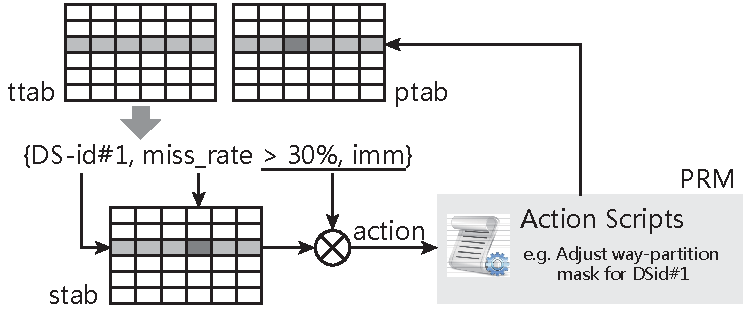
\includegraphics[width=0.7\textwidth]{hwres/trigger-action-flow}
  \caption{``\emph{trigger$\Rightarrow$action}''编程方法示意图}
  \label{fig:trigger-action-flow}
\end{figure}

如图\ref{fig:trigger-action-flow}所示,trigger是基于状态表中某一统计信息(如IPC、缺失率、延迟等)的触发条件,
action是对针对该触发条件所执行的动作,因此action也可以被称做是trigger-handler。
触发条件保存在控制平面的触发表中,而与之对应的action动作则是由系统管理员编写,并存储在PRM的固件中。
系统管理员可以为每个应用标签设定不同的``\emph{trigger$\Rightarrow$action}''规则,
以实现不同的资源管理策略。

由于action动作是运行在PRM固件内,因此可以使用任何语言来编写,
并通过PRM提供的方法使其于触发条件建立关联,并在触发条件满足时自动调用。
同时,由于PRM可以控制系统内所有的控制平面,trigger和action可以针对不同的硬件资源进行设定。
例如,可以设定一个监控访存带宽的触发条件,但它的触发动作却是调整共享末级缓存的容量,
以此影响其命中率,进一步实现访存带宽的调整。
通过这种跨硬件资源的触发规则,可以实现更为灵活的节点内硬件资源协同管理。

根据应用的需求为每个应用编写适当的触发规则是一个十分复杂的工作,
但数据中心管理员可以根据不同的资源管理策略,
预定义多种不同的``\emph{trigger$\Rightarrow$action}''触发规则与动作,
并依此为用户提供不同级别的SLA(Service-Level Agreements)。
用户根据自己的QoS需求选择合适的SLA,通过这些预定义的触发规则与动作来满足其QoS需求。

%本节所描述的``\emph{trigger$\Rightarrow$action}''编程方法与上一节所描述的资源监控与管理的编程接口
%将在第\ref{chap:prm}中进行统一介绍。

\subsection{通用控制平面微体系结构设计}
\label{chap:hwresman:cp:uarch}

综合以上控制平面功能与设计,其微体系结构如图\ref{fig:pard-cp-design}所示。
PARD控制平面的核心是3个控制表,即参数表、状态表和触发表。
参数表与硬件模块之间通过参数接口(HW PARAM IF)进行交互,
硬件在收到请求后,使用请求中的应用标签DS-id查询参数表,获取需要的参数;
状态表与硬件模块之间通过状态接口(HW STAT IF)进行交互,
硬件在完成每一个请求后,通过该接口实现状态的更新。
除此之外,控制平面中还包含连接控制平面网络的接口模块,
PRM通过该模块来访问3个控制表。

3个控制表都使用CAM+RAM的结构实现,
其中参数表与统计信息表的CAM中使用应用标签DS-id进行索引,
触发表的CAM中除应用标签DS-id外还包括触发条件对应的统计信息编码。
参数表在收到参数查询请求后,通过CAM查询该请求所对应的表项,
并在RAM中获取其参数并返回给硬件模块;
统计信息表的更新过程与参数表类似,通过CAM查询表项,将新的统计信息更新到RAM对应的表项中;
在统计信息表更新的同时,应用标签和统计信息编码同样被送到触发表的CAM中,
用于查询是否存在与本次更新相对的触发条件,如果触发条件存在且满足,
则通过CPN接口模块向PRM发送触发事件通知。

\begin{figure}[tb]
  \centering
  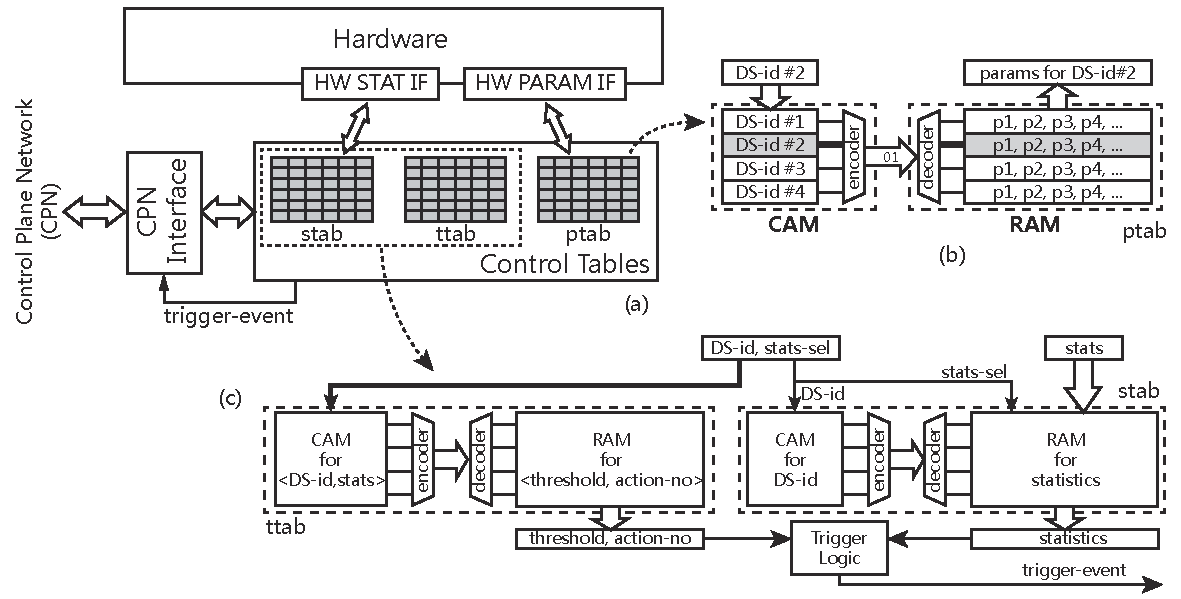
\includegraphics[width=\textwidth]{hwres/pard-cp-design}
  \caption[控制平面微体系结构设计]{控制平面微体系结构设计:
  (a)控制平面的核心是3个控制表,即参数表ptab、统计信息表stab和触发表ttab,
       以及这3个控制表与控制平面网络和硬件设备的接口模块;
  (b)参数表由CAM和RAM组成,实现按DS-id索引参数的功能;
  (c)统计信息表与触发表同样由CAM和RAM组成,触发表的CAM按<DS-id, stats>组合索引,
       该图为统计信息表更新以及触发检查逻辑。}
  \label{fig:pard-cp-design}
\end{figure}

控制平面网络接口模块使用寄存器窗口的方式对外提供控制表的访问,
如图\ref{fig:pard-cp-intf}所示。
系统内所有的控制平面都被映射到一段连续的16位I/O地址空间中(64KB),
每一个控制平面在其中使用32个字节用于映射其控制寄存器,控制寄存器的定义如图\ref{fig:pard-cp-intf}所示。
其中IDENT和IDENT\_HIGH 2个寄存器(总计12字节)存储该控制平面的名字,
type寄存器表示该控制平面的类型,
address/cmd/data 3个寄存器用于实现对控制平面中控制表的访问。
其中address寄存器包含16位的逻辑域标签DS-id、2位的控制表选择、以及14位的列偏移,
通过该寄存器实现对控制表项的寻址,而cmd寄存器用于指定对该控制表项的操作,
当前的实现中只包含读、写两种类型的操作。
对于写操作,用户需要提前将数据写入到data寄存器,而对于读操作data寄存器的写入操作由控制平面硬件完成,
用户可以从该寄存器中读取所选择的控制表项内容。

PRM通过以上描述的寄存器接口实现对控制平面的编程,具体流程如下:
控制平面驱动首先将目标表项的地址写入到地址寄存器,其中包括逻辑域标签DS-id(行)以及表项偏移(列)。
如果用户的操作是修改表项,则驱动首先将新的表项写入到data寄存器,然后在命令寄存器中写入WRITE命令;
如果是对表项的查询操作,则直接向命令寄存器写入READ命令,并在操作完成后从data寄存器中读取数据。

\begin{figure}[tb]
  \centering
  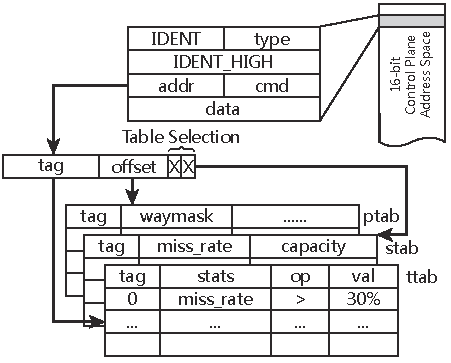
\includegraphics[width=0.5\textwidth]{hwres/pard-cp-intf}
  \caption[控制平面接口]{控制平面接口}
  \label{fig:pard-cp-intf}
\end{figure}


\subsection{控制平面示例}

本节将以处理器末级缓存和内存控制器为例,介绍如何将控制平面集成到硬件部件中,
图\ref{fig:pard-cache-cpdesign}和图\ref{fig:pard-mig-cpdesign}是已经增加了控制平面的微体系结构示意。
对比这两者可以发现,其控制平面具有相同的结构,只是控制表的内容存在差别,
该通用的控制平面结构可以很容易的集成到不同的硬件部件中,而只需要对其控制表及硬件接口部分进行修改。

\textbf{共享末级缓存控制平面}\quad
图\ref{fig:pard-cache-cpdesign}是共享末级缓存控制平面的微体系结构示意图,
其支持可编程的路划分机制,借助这一机制可以为应用程序调整Cache容量。
该控制平面由3个基本的控制表组成,即参数表、统计表以及触发表,
这三张控制表可以通过可编程接口由PRM上的固件进行访问;
控制平面同时还包括一个连接到PRM的中断线。
除了引入控制平面以外,还需要对原有缓存控制器中的Tag Array以及伪LRU逻辑进行了修改,
所有这些修改均以阴影和虚线的方式在图中进行了标识。

\begin{figure}[tb]
  \centering
  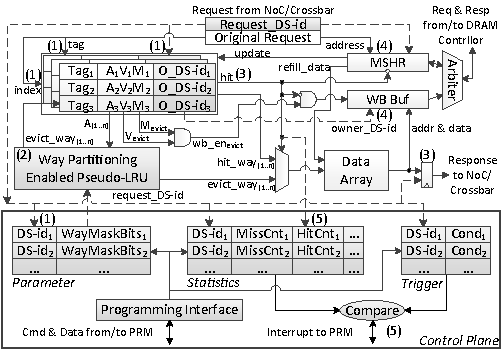
\includegraphics[width=0.7\textwidth]{hwres/pard-cache-cpdesign}
  \caption{共享末级缓存控制平面}
  \label{fig:pard-cache-cpdesign}
\end{figure}

控制平面的引入是否会为共享末级缓存带来额外的延迟是在设计过程中需要考虑的重要问题,
幸运的是目前系统中Cache控制器都是基于流水线设计,
这就使得控制平面的逻辑开销能够隐藏在原有的流水线中,具体流程如下:

\begin{enumerate}[leftmargin=2\parindent, nolistsep, label=(\arabic*)]
  \item 当一个包含DS-id和地址的Cache访问请求到达控制器时,
        首先需要利用DS-id从参数表中获得相应的路划分掩码。
        例如掩码``0x00FF''代表在整个16路中仅使用低端的8路。
        与此同时,请求地址被用来在Tag Array中查找相应的条目,
        这些条目除了普通的Tag和状态信息以外,还保存有DS-id;
  \item 伪LRU逻辑利用参数表输出的掩码以及Tag Array输出的访问历史计算出哪一路需要被替换;
  \item 如果请求在缓存中命中,那么数据将从Data Array中取回,
        连同请求的DS-id一起通过NoC或者crossbar返回给CPU。
        需要注意的是,缓存的命中条件发生了改变,除了请求地址与条目Tag之间原有的约束以外,
        还需要请求DS-id与条目DS-id相互匹配。
  \item 如果请求在缓存中没有命中,Cache控制器会分配一个MSHR条目,
        并在该条目中保存原始请求及其DS-id。
        当被请求的数据返回时,Cache控制器需要将MSHR中保存的原始请求DS-id写入到TagArray中。
        该DS-id作为``owner DS-id'',在脏数据写回时,
        需要与地址和数据一同送入回写缓存,并发送到内存控制器。
  \item 在以上各个步骤的过程中,Cache控制平面还会完成以下若干操作:
        更新统计表,将Cache使用统计数据发送给平台资源管理器,
        在必要时激活触发条件并发出一个中断信号给PRM。
        需要特别指出的是这些操作并不在关键路径上,不会对延迟造成影响。
\end{enumerate}

%可编程接口用于PRM固件访问该控制平面的3个控制表,
%它首先从PRM接收控制表的访问命令,选择相应的表并从指定的表项中读取或写入数据,
%更多细节请参见第\ref{chap:prm}章。

\textbf{内存控制器控制平面}\quad
图\ref{fig:pard-mig-cpdesign}是内存控制器控制平面的微体系结构示意图,
为了让PARD的逻辑域抽象能够运行未经修改的操作系统和应用,
该控制平面的参数表保存了用于逻辑域物理地址与DRAM地址的映射信息。
除此之外,控制表中还保存了每个逻辑域的优先级信息用于访存调度。

\begin{figure}[tb]
  \centering
  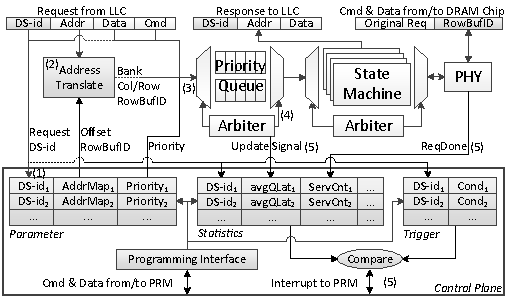
\includegraphics[width=0.7\textwidth]{hwres/pard-mig-cpdesign}
  \caption{内存控制器控制平面}
  \label{fig:pard-mig-cpdesign}
\end{figure}

%Regarding performance isolation, unlike the LLC, the memory
%control plane needs to takes into account two factors, i.e., queuing
%delay and row buffer locality. To manage queuing delay, we add
%a priority queuing mechanism into the memory controller. The
%number of queues depends on the priority levels supported by
%the memory control plane. Our current design only supports two
%priories, but it is easy to extend. To avoid memory low-priority
%requests degrading the row buffer hit rate of high-priority requests,
%we add one extra row buffer into each DRAM chip for high-priority
%memory requests. If we want to augment DRAM chip with more
%buffers, we can leverage some commercial designs such as NEC’s
%virtual-channel memory (VCM).

在性能隔离方面,与Cache控制面不同的是内存控制器控制平面需要考虑以下2个因素:
排队延迟和行缓冲(row buffer)局部性。
为了管理排队延迟,PARD在内存控制器中加入了优先级队列机制,
队列数目取决于内存控制平面能够支持的优先级等级。
当前的设计中暂时仅支持2个优先级,但可以很容易被扩展到多个优先级。
为了防止低优先级访存请求干扰并降低高优先级访存请求的行缓冲命中率,
在DRAM芯片中为高优先级内存请求增加了一个额外的专用行缓冲。
如果需要为DRAM芯片增加更多的优先级控制能力,
可以参考NEC的virtual-channel memory(VCM)\cite{nec-vcm}技术。

在添加了以上机制后,当一个带有DS-id的内存访问请求到达内存控制器时,
将会顺序引发下列操作:

\begin{enumerate}[leftmargin=2\parindent, nolistsep, label=(\arabic*)]
  \item 控制平面利用请求的DS-id从参数表中获得与之相应的地址映射信息、
        队列优先级以及行缓冲编号;
  \item 请求逻辑域物理地址被转换成DRAM物理地址;
  \item 根据控制表中获取的优先级信息将请求连同DS-id置入相应的请求等待队列中;
  \item DRAM调度器根据高优先级优先以及FR-FCFS\cite{rixner_memory_2000}策略从等待队列中选取请求进行服务;
  \item 控制平面更新统计表并检查是否满足触发条件,如果满足则发送中断信号到PRM。
\end{enumerate}

\subsection{模拟器实现与评测}

本节在第\ref{chap:labeladdrspace:nohype}节所建立的模拟器基础上,
按照本章所述方法对处理器末级缓存和磁盘控制器进行改造,包括:
1)在处理器末级缓存中增加缓存容量划分功能,
2)在磁盘控制器中增加基于带宽划分的调度功能。
并为它们增加控制平面,同时在模拟器中模拟了基于X86-SoC的PRM,
实现对这2个硬件资源的集中式管理。

修改后的模拟器最多支持启动4个逻辑域,
能够通过PRM调整4个逻辑域对处理器末级缓存与磁盘控制器的资源分配,
本节将使用该模拟器验证控制平面对资源分配的控制(磁盘控制器)、
以及``\emph{trigger$\Rightarrow$action}''机制的效果(处理器末级缓存)。
%更多模拟器的实现细节将在第\ref{chap:impl:simulator}节中进行介绍。


\subsubsection{``\emph{trigger$\Rightarrow$action}''机制验证}

本节利用``\emph{trigger$\Rightarrow$action}''机制解决应用服务质量与服务器资源利用率冲突的问题,
实验场景与配置如图\ref{fig:hwres-sim-config}所示:
一台4核的PARD服务器被划分为4个逻辑域,其中LDom\#0中运行延迟敏感型应用memcached,
其他3个逻辑域中运行批处理应用,考察资源共享对延迟敏感型应用性能的影响。

\begin{figure}[tb]
  \centering
  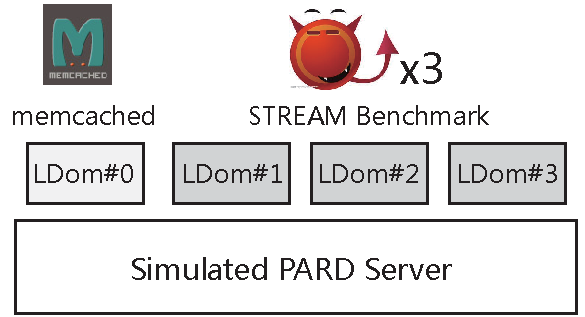
\includegraphics[width=0.5\textwidth]{hwres/hwres-sim-config}
  \caption{``\emph{trigger$\Rightarrow$action}''机制验证实验配置}
  \label{fig:hwres-sim-config}
\end{figure}

由于模拟器本身的模拟速度非常慢,增加网络环境模拟会进一步降低模拟速度,
因此在实验时将memcached服务器与客户端运行在同一个逻辑域中,它们共享一个CPU核心。
虽然服务器和客户端会在同一个逻辑域内发生资源竞争,
但由于本文更多关注的是逻辑域(应用)之间的干扰,因此这种黑箱内部的竞争是可接受的。
本实验使用STREAM benchmark\cite{stream}作为批处理应用,
该benchmark会在处理器末级缓存产生严重的干扰,因此可以使实验效果更加明显。

实验分为两步,
首先使用模拟器的simple-timing模型来启动Linux操作,启动应用并建立checkpoint;
然后使用Out-Of-Order(O3)模型恢复该checkpoint,最后的实验评估使用O3模型进行。
受到模拟速度的影响,本实验只模拟了memcached应用的3秒钟执行(花费大约30个小时),
其中第1秒是warm-up过程,后2秒才被用于评估。

图\ref{fig:pardsim:memcached-resptime}展示了在不同请求负载下memcached的长尾响应时间。
当memcached单独运行时(图中solo曲线),它能够满足22.5KRPS的请求负载,
同时长尾(95\%-tail)响应时间也是在合理的范围(0.6ms)。
然而,由于只1个处理器核在运行,此时服务器的利用率仅为25\%。
如果另外3个逻辑也被启动运行,并与memcached所在的逻辑域共享资源,
整个服务器达到100\%的利用率,
但此时memcached的性能下降到15KRPS,并且长尾响应时间也超过了1ms。
如果进一步提高请求负载到20KRPS,长尾响应时间增加超过2个数量级(62.6ms)。

为了验证``\emph{trigger$\Rightarrow$action}''机制的效果,
预先在PRM中为memcached所在的逻辑域LDom\#0定义了与图\ref{fig:trigger-action-flow}
类似的触发规则:
\begin{verse}
``\emph{LLC.MissRate $>$ 30\% $\Rightarrow$ 增加LLC容量到全部容量的50\%}''
\end{verse}

在启动所有的逻辑域前,将以上规则安装到处理器末级缓存控制平面中,
图\ref{fig:pardsim:memcached-20krps-missrate}给出了实验过程中收集的处理器末级缓存缺失率,
从图中可以看到当3个干扰应用运行后,memcached的缓存缺失率显示上升,
并达到了规则设定的触发阈值(30\%),控制平面应用action动作,
将一半的缓存容量划分给memcached所在的逻辑域,在此之后memcached的缓存缺失率显著下降,
降低到10\%左右,只略高于单独运行时7\%的缺失率。
最终在22.5KRPS的请求速率下,长尾响应时间只有1.2ms,
由于memcached所能使用的处理器末级缓存只有单独运行时的一半,
因此其长尾响应时间要略高于单独运行时的响应时间。

以上实验结果表明,即使4个处理器核全部都在工作,服务器资源利用率为100\%的情况下,
memcached的性能仍然没有受到严重的影响。
这证明``\emph{trigger$\Rightarrow$action}''机制能够利用PARD提供的硬件资源管理功能,
实现服务器资源利用率与应用服务之间的平衡。

\begin{figure}[tb]
\begin{minipage}{0.48\textwidth}
  \centering
  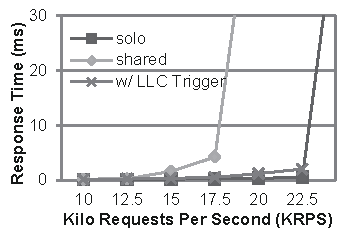
\includegraphics[height=4.5cm]{hwres/pard-sim-memcached-resptime}
  \caption{模拟器memcached 95\%-tail延迟示意图}
  \label{fig:pardsim:memcached-resptime}
\end{minipage}\hfill
\begin{minipage}{0.48\textwidth}
  \centering
  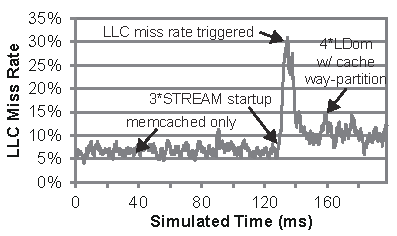
\includegraphics[height=4.5cm]{hwres/pard-sim-memcached-20krps-missrate}
  \caption{模拟器memcached末级缓存命中率变化(20KRPS)}
  \label{fig:pardsim:memcached-20krps-missrate}
\end{minipage}
\end{figure}


\subsubsection{磁盘I/O带宽控制}

PARD控制平面不仅能管理处理器末端级缓存这类基于容量的资源,
同时能够管理基于流量的资源,如内存带宽与I/O带宽。
本节验证控制平面对带宽的控制,这里使用磁盘I/O带宽作为实验目标。

在本节的实验中,只使用模拟器中2个逻辑域,在其中使用命令
``\textit{dd if=/dev/zero of=/dev/sdb bs=}32\textit{M count=}16''
执行磁盘写操作。
初始状态下,2个逻辑域共享磁盘控制器且具有相同的优先级,由于它们执行的命令与参数完全相同,
因此2个逻辑域所得到的磁盘I/O带宽完全相同。
此时假设逻辑域LDom\#0的用户需要得到更好的I/O性能,例如云计算场景下通过更高的费用获取更快的性能,
管理员可以在PRM内执行以下命令重新调整服务器中磁盘I/O带宽的分配,将80\%的带宽分配给该用户。
\begin{verse}
\textit{echo} 80 \textit{$>$ /sys/cpa/cpa}3\textit{/ldom}0\textit{/parameters/bandwidth}
\end{verse}

该命令通过PRM对磁盘控制器控制平面(cpa3)进行编程,修改LDom\#0的带宽占比为80\%,
图\ref{fig:pardsim:iosched}给出了磁盘I/O带宽分配的效果。

虽然诸如cgroup\cite{cgroup}之类的方法也能提供类似的I/O带宽管理功能,
但PARD所提供的资源管理方法能够在硬件层次实现更为细粒度的资源管理,
同时无需对用户操作系统或应用进行任何的修改,降低了软件栈的复杂度与开销。
关于控制平面的编程接口,以及如何在PRM中实现资源管理将在第\ref{chap:prm}章进行详细的介绍。

\begin{figure}[tb]
  \centering
  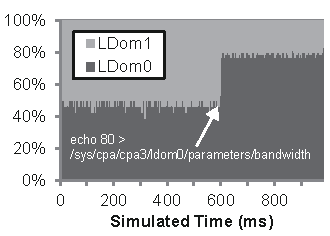
\includegraphics[width=0.45\textwidth]{hwres/pard-sim-iosched}
  \caption{磁盘I/O性能隔离}
  \label{fig:pardsim:iosched}
\end{figure}


\section{可编程数据平面设计}
\label{chap:hwresman:dp}

正如本章引言所述,PARD的硬件资源管理机制包括控制平面与数据平面两部分,
上一节已经对控制平面接口功能进行描述,
本节主要针对数据平面的需求设计可编程数据平面,具体包括:
数据平面处理器的设计、资源管理机制的集成、以及数据平面可编程的实现。

%需要能够适应不同的硬件,并为控制平面提供统一的管理接口;
%能够提供灵活的可编程机制;
%能够很容易的集成现有资源管理相关工作。
%
%可编程技术目前主要包括两类,一类是以FPGA为代表的硬件可编程,一类是使用处理器实现软件。
%
%基于xxxx的考虑,本文使用基于处理器的实现。
%
%另一方面,控制平面的``\emph{trigger$\Rightarrow$action}''机制在响应时间上存在瓶颈:
%每当触发条件发生后,需要经过控制平面网络将该事件传递到PRM,
%由运行在PRM中的软件代码来更新策略,并通过控制平面网络写回到控制平面中。
%由于受到控制平面网络延迟以及PRM软件代码延迟的影响,
%该机制并不能达到特别高的响应速度。
%同时并非所有的触发条件发生后都需要在PRM进行全局处理,
%完全可以预定义一些动作,在控制平面本地完成处理。
%
%本节后续内容将对数据平面处理器的设计以及资源管理机制的集成进行介绍,
%最后介绍数据平面运行时可编程的实现。

\subsection{数据平面处理器体系结构}

\begin{figure}[tb]
  \centering
  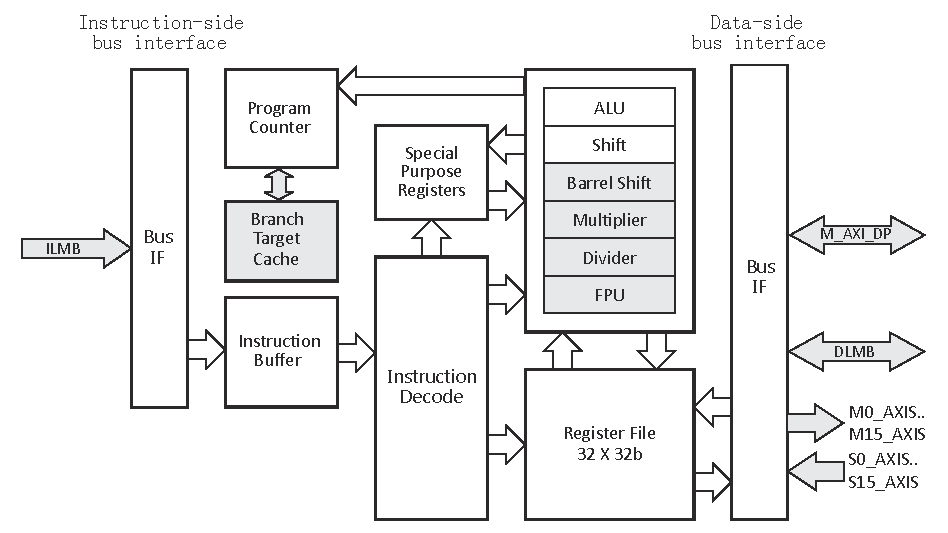
\includegraphics[width=0.8\textwidth]{hwres/pard-dp-proc}
  \caption{数据平面处理器结构图}
  \label{fig:pard-dp-proc}
\end{figure}

由于数据平面处理器位于请求处理的关键路径上,为了保障系统的性能不受影响,需要从以下3个方面进行考虑:

\begin{enumerate}[leftmargin=2\parindent, nolistsep, label=\arabic*)]
  \item 处理器需要执行一系列指令才能完成对请求的处理,因此处理器需要工作在比其所在硬件部件更高频率,以满足硬件部件的性能需求;
  \item 处理器的固件代码执行需要确定性,因此不能使用cache结构,而是使用scratchpad memory代替;
  \item 由于高频需求,因此处理器功能要尽可能简单,一些必需的复杂的逻辑(如数据压缩与加密等)通过外部加速器的方式进行扩展。
\end{enumerate}

基于以上需求,本文最终选择使用RISC作为数据平面处理器的基础架构,如图\ref{fig:pard-dp-proc}所示,并对其进行修改以适应数据平面处理器的需求。
包括:1)架构精简,只保留其基本功能,以满足频率需求;
2)增加scratchpad memory作为指令与数据存储;
3)增加请求缓存接口用于接入硬件设备中;
4)增加控制平面接口用于连接控制平面。
由第\ref{chap:hwresman:res}节可知,对于内存控制器与处理器末级缓存,该处理器的主要工作包括:
对请求进行调度、地址变换,对数据进行处理,生成控制信号(如Cache缓存与替换)。
要完成以上工作,该处理器需要具备基本的处理器功能外,还需要在数据类型、存储模型和指令上进行扩展。

\subsubsection{数据类型}

数据平面处理器中执行的算法代码大都只是对输入的请求进行处理,
因此该处理器只有``无符号整数''和``请求''两种数据类型,如图\ref{fig:pard-dp-datatype}所示。
无符号整数的长度与处理器的位宽相同,都被设置为其所属硬件的位宽,
以节约请求处理时位宽转换的开销,保障请求处理的效率。

\begin{figure}[b]
  \centering
  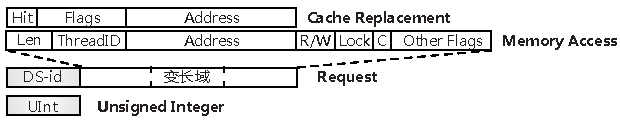
\includegraphics[width=0.7\textwidth]{hwres/pard-dp-datatype}
  \caption{数据平面处理器支持的数据类型}
  \label{fig:pard-dp-datatype}
\end{figure}
 
``请求''类型的是一个变长数据类型,其中包含了固定的16位应用标签(DS-id)以及变长的请求数据。
以访存请求为例,其中包含请求地址、长度、线程号、读写类型、锁与缓存状态等其他一些标志位;
对于Cache替换请求,其中包含了请求地址、Hit/Miss标记以及其他一些标志位等信息。
图\ref{fig:pard-dp-datatype}给出了访存请求以及Cache替换请求类型的示例。
数据平面处理器本身并不关心请求类型中具体每个位的意义,而只是将其做一个整体进行处理,
对每个域的解析或修改由其运行的固件代码完成。

\subsubsection{存储模型}
数据平面处理器中程序员可见的存储结构包含寄存器、请求缓存、scratchpad memory、I/O地址空间四部分。
与传统的RISC架构相同,数据平面处理器包含32个通用寄存器(\textit{r}0-\textit{r}31),
用于进行算数逻辑运算,其中\textit{r}0是常数0;
除此之外,增加了4个用于保存``请求''类型数据的请求寄存器(\textit{s}0-\textit{s}3),
可以通过请求缓存操作指令(rbget和rbput,参见第\ref{chap:hwresman:dp:isa}节),
将请求输入队列中的请求读取到该寄存器、或将该寄存器中的请求加入到请求输出队列中;
请求寄存器不能直接参与算术逻辑计算,需要先将其部分数据读取到通用寄存器后才能执行计算;
请求寄存器之间可以直接进行数据交换。
处理器执行的固件代码与数据保存在scratchpad memory中,需要用户自行管理。
控制平面被映射为数据平面处理器的外设,提供处理器的固件代码ROM以及处理器的对外接口。

\subsubsection{指令集}
\label{chap:hwresman:dp:isa}

数据平面处理器使用RISC标准的算数逻辑、控制流和访存指令,
并在其基础上额外增加了请求缓存操作指令。

请求缓存分为两部分,一个输入缓存一个输出缓存。
其中输入缓存既可作为FIFO操作,也可基于DS-id进行内容寻址;
输出缓存只能作为FIFO操作。
用于请求缓存操作的指令如表\ref{tab:pard-dp-isa}所示,
指令rbput可以将指定请求寄存器中的请求添加到输出缓存队列末尾;
指令rbget有两种使用方式,一种是将输入缓存作为FIFO,取出队列头的请求到请求寄存器,
另一种是通过DS-id对请求进行筛选,取出第一个满足应用标签的请求到请求寄存器。
指令rbcp用于在请求寄存器之间传送数据。
指令mfrb用于将请求寄存器中的部分数据传送到通用寄存器;
指令mtrb与之相反,用于将通用寄存器的数据传送到请求寄存器指定的位置。

% 数据平面处理器扩展指令
\begin{table}[htb]
  \centering
  \begin{minipage}[t]{0.95\linewidth}
  \caption{数据平面处理器扩展指令}
  \label{tab:pard-dp-isa}
    \begin{tabular*}{\linewidth}{lll}
      \toprule[1.5pt]
      {\heiti 指令} & {\heiti 用途} \\
      \midrule[1pt]

      \multirow{2}{*}{\textbf{rbput}} & \multicolumn{2}{l}{将请求寄存器中的请求增加到请输出请求缓存FIFO队尾。示例:}                               \\
                                      & rbput \textit{rb}0, \textit{s}0 & \#将\textit{s}0加入到\textit{rb}0队尾                                    \\
      \hline
      \multirow{3}{*}{\textbf{rbget}} & \multicolumn{2}{l}{从输入请求缓存读取一个请求到指定的请求寄存器。示例:}                                   \\
                                      & rbget \textit{s}0, \textit{rb}0                & \#从\textit{rb}0获得第1个请求到\textit{s}0寄存器          \\
                                      & rbget \textit{s}0, \textit{rb}0, \textit{DSid} & \#从\textit{rb}0获得第1个\textit{DSid}为给定值的请求到\textit{s}0寄存器 \\
      \hline
      \multirow{2}{*}{\textbf{rbcp}}  & \multicolumn{2}{l}{请求缓存寄存器之间传递数据}                                                             \\
                                      & rbcp \textit{s}0, \textit{s}1                  & \#将\textit{s}1的值传递给\textit{s}0                      \\
      \hline
      \multirow{3}{*}{\textbf{mfrb,mtrb}}   & \multicolumn{2}{l}{请求缓存寄存器与通用寄存器之间传递值。示例:}                                     \\
                                      & mfrb \textit{r}4, \textit{s}0, 0               & \#将\textit{s}0第1个32位数据送到\textit{r}4寄存器         \\
                                      & mtrb \textit{s}1, \textit{r}5, 1               & \#将\textit{r}5寄存的数据送到\textit{s}1寄存器第2个32位   \\
      \bottomrule[1.5pt]
    \end{tabular*}\\[2pt]
  \end{minipage}
\end{table}

\subsection{固件代码示例}
本节将以3段不同功能的固件代码为例,介绍数据平面处理器的编程方法。

\textbf{段式地址映射}\quad
本示例用于实现PARD的内存控制器控制平面所提供的地址映射功能,
该功能只需要对访存请求的地址进行修改,而请求的数据无需修改,
因此将地址与数据分开由2个处理器进行处理,
如图\ref{fig:pard-dp-ex-mapping}所示。
对于数据处理器,其固件代码只使用rbget/rbput指令对请求进行转发。
地址处理器首先需要使用rbget指令获取当前请求到请求寄存器,
并使用mfrb指令将其中的地址与DSid读取到通用寄存器;
而后通过查表的方式获得该请求对应的映射目的地址的基址,
对请求地址进行变换,并使用mtrb指令将变换后的地址写回到请求寄存器,
最后通过rbput指令将新的访存请求从处理器中送出,完成地址映射功能。

\begin{figure}[H]
  \centering
  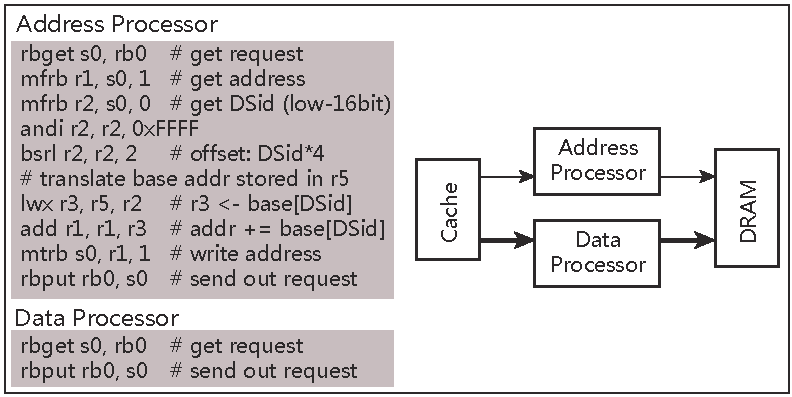
\includegraphics[width=0.7\textwidth]{hwres/pard-dp-ex-mapping}
  \caption{段式地址映射示例}
  \label{fig:pard-dp-ex-mapping}
\end{figure}
 
\textbf{数据加密}\quad
本示例实现访存数据加密功能,由于数据加密操作通常需要耗费很长的时间,
而且数据平面处理器提供的指令集并不足以完成该操作。
因此在处理器外部实现了硬件AES加密模块,并通过请求接口将其连接到数据平面处理器上,
该结构如图\ref{fig:pard-dp-ex-aes}所示。
基于该结构,数据处理器只需要将数据发送到AES模块并等待其完成加密,
将加密后的数据送出处理器即可。
数据解密与加密过程类似,只需将数据发送到连接有解密模块的请求接口即可。

\begin{figure}[H]
  \centering
  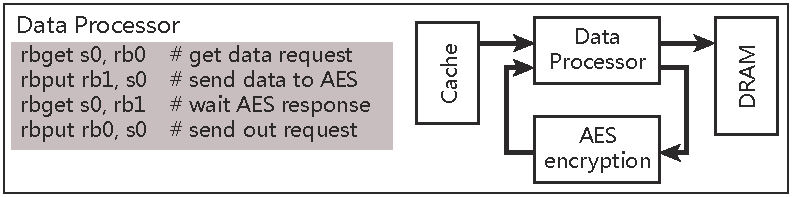
\includegraphics[width=0.7\textwidth]{hwres/pard-dp-ex-aes}
  \caption{访存数据加密示例}
  \label{fig:pard-dp-ex-aes}
\end{figure}
 
\textbf{缓存替换策略}\quad
本示例实现缓存替换策略功能,使用可编程处理器替换Cache中原有的LRU模块,
使用软件实现基于二叉树的伪LRU替换策略。
如图\ref{fig:pard-dp-ex-cache}所示,处理器固件代码工作流程如下:
1)处理器收到Cache前端的请求后,以及Hit/Miss信息,如果缓存命中则无需任何额外操作;
2)对于缓存缺失的请求,首先从地址中解析出tag与set信息,
并将解析后的set地址发送到Tag Array,等待其返回该set的信息;
3)根据TagArrary返回的set信息,以及内部的数据结构生成替换目标;
4)将替换目标送出处理器。

\begin{figure}[H]
  \centering
  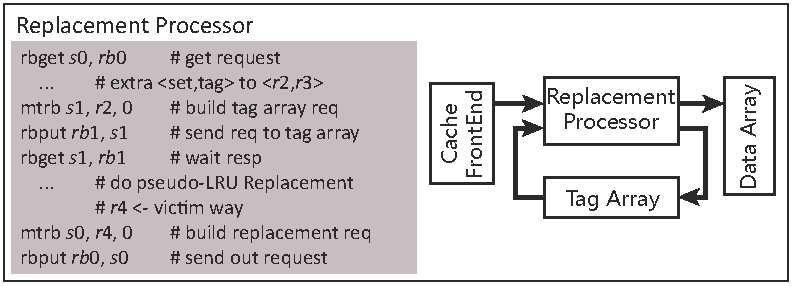
\includegraphics[width=0.7\textwidth]{hwres/pard-dp-ex-cache}
  \caption{缓存替换策略示例}
  \label{fig:pard-dp-ex-cache}
\end{figure}


\subsection{可编程支持}

数据平面的可编程主要体现在数据平面处理器的固件代码更新,
通过更新固件代码的方式实现策略的调整。
对数据平面处理器固件代码更新可以分为兼容性更新与非兼容性更新,
其中``兼容性''是指更新前后的代码是否对数据平面的功能产生更改。
对于非兼容性更新,需要首先关闭系统中所有正在运行的逻辑域,
并在数据平面处理器固件更新完成后重新启动逻辑域;
对于兼容性更新,系统可实现无中断运行,
但需要对数据平面处理器与硬件的接口处进行额外的处理,
如图\ref{fig:pard-dp-fw-upgrade}所示。

\begin{figure}[htb]
  \centering
  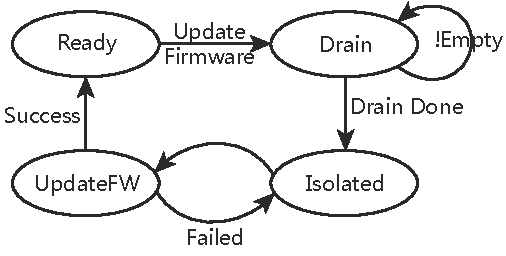
\includegraphics[width=0.6\textwidth]{hwres/pard-dp-fw-upgrade}
  \caption{数据平面处理器兼容性固件更新状态图}
  \label{fig:pard-dp-fw-upgrade}
\end{figure}

在收到更新固件命令后进入Drain状态,阻止请求继续发送到数据平面处理器,
等待数据平面处理器处理完全部请求,并将请求队列排空后,使处理器进入Isolated隔离状态;
之后完成对固件代码的更新,新的固件代码开始运行后,开始进行初始化操作,
其中包括旧固件的状态数据迁移步骤;
在所有的初始化操作完成后,处理器恢复到就绪状态,重新开始处理请求,
至此完成数据平面处理器固件代码的兼容性更新操作。


\section{小结}

本章介绍了PARD体系结构中硬件资源共享管理方法与架构,
包括硬件资源的``数据平面''与``控制平面''抽象,及其具体的实现。
控制平面通过控制表实现,为用户提供了资源管理接口,
同时提出了``\emph{trigger$\Rightarrow$action}''编程方法,
基于模拟器的实验结果表明,该方法与PARD提供的资源管理机制结合,
能够实现数据中心服务器资源利用率与应用服务质量的平衡。
针对数据平面可编程需求,本章提出一种数据平面处理器设计,
并将其应用到处理器末级缓存与内存控制器数据平面中,
通过软件编程的方式实现硬件资源管理的扩展。

